\documentclass{article}
\usepackage{amsmath, amssymb, cite, algorithmic, url, braket}
\usepackage{graphicx}
\usepackage{pythonhighlight}
\usepackage[margin=1.5cm]{geometry}
\usepackage[title]{appendix}
\usepackage{subfigure}
\usepackage{listings}
\usepackage{booktabs}

\graphicspath{{../pic/}}
\lstset{
language=[ANSI]{C},
showtabs=true,
tab=,
tabsize=2,
basicstyle=\ttfamily\footnotesize,%\setstretch{.5},
stringstyle=\color{stringcolour},
showstringspaces=false,
alsoletter={1234567890},
otherkeywords={\%, \}, \{, \&, \|},
keywordstyle=\color{keywordcolour}\bfseries,
upquote=true,
morecomment=[s]{/*}{*/},
commentstyle=\color{commentcolour}\slshape,
literate=*%
{=}{{\literatecolour=}}{1}%
{-}{{\literatecolour-}}{1}%
{+}{{\literatecolour+}}{1}%
{*}{{\literatecolour*}}{1}%
{!}{{\literatecolour!}}{1}%
{[}{{\literatecolour[}}{1}%
{]}{{\literatecolour]}}{1}%
{<}{{\literatecolour<}}{1}%
{>}{{\literatecolour>}}{1}%
% {>>>}{\pythonprompt}{3}%
,%
frame=trbl,
rulecolor=\color{black!40},
backgroundcolor=\color{white},
breakindent=.5\textwidth,frame=single,breaklines=true
}

\begin{document}
\title{DSP Homework 09}
\author{Xu, Minhuan}
\maketitle
\tableofcontents
\begin{abstract}
\subsubsection*{videos}
After summing up the videos, I learned more about them.
\subsubsection*{Digital Number Representations}
I found out the specific definition of digits number representations and made my proposal.
\subsubsection*{Lloyd-Max Quantization Algorithm}
I quantized a picture with Lloyd-Max Quantization Algorithm.
\subsubsection*{Optimal Quantization Strategy When PDF Has Uniform Distribution}
I found the Optimal Quantization Strategy When PDF Has Uniform Distribution.
\end{abstract}

\section{Videos}
\subsection{Analog Resurgence}

\subsubsection{Background}
The analog computers are born earlier than their digital relatives, they are powerful facing complex calculations, but since the continuous values are not measurable and repeatable, analog computers don't have the capability of doing calculations which need high precision. Also, the analog devices vary along with temperature, production technique and even time, and the digital computers eventually take responsibility of mostly calculations today.

\subsubsection{Neural Network}
Our neurons get zero-one input from many other neurons, and each of the input has their own weight. Than, these inputs go through an process much like the weighted average to get a result, and if the result is large enough, the neuron outputs one, vice-versa.

The first neural-network-like thing perceptron is created in the last century. The perceptron are used to judge what in the picture. 
The pictures are actually pixel matrix, and each pixel can be seen as a neuron which has an activation between $[0, 1]$, these neurons are connected into a output neuron. Then, they trained the perceptron by increase or decrease the weights the output neuron hold in specific areas according to \emph{something} so that this perceptron can judge the \emph{thing} in front of it is or isn't that \emph{something}.

We can find that perceptron needed to do the matrix multiplication during judging things. Also, in this video, they animated the process, that is
\begin{enumerate}
	\item Flatten the image pixel to a matrix $\mathcal{A}$ with 1 row and N (total quantity of pixels) cols.
	\item Multiply $\mathcal{A}$ with a matrix with N rows and 1 col, and the result is just a number.
	\item Compare the result with a certain number, and decide whether the output is zero or one.
\end{enumerate}

\subsubsection{Actual Analog Chips Applied to Neural Network}

This kind of chips are like the EEPROM, if we change the amount of electronics in the Gate of FET, the resistance between the Drain and Source will change as well. Here, they carefully designed the FET so that the resistance mentioned is linear to the electronics in the Gate. Therefore, multiplication of real numbers can be represented as below

$$
	current = conductance \times voltage
$$

If they arrange the FETs in the way of matrix, they can do matrix multiplication as well. That's amazing.

\subsection{New Brain Cells}
Actually, the speaker told us that our brain are producing new neurons in the hippocampus during our whole life. This phenomena is called neurogenesis. 

According to the researches neurologists did, this action of producing new neurons is associated with people's learning abilities, memory, mood and emotion. The more neurons are produced, the better we learn and remember things.

Moreover, the so-called neurogenesis happening in everybody is a target of choice of our body. If we do sports,learn, eat regularly, be happy, there will be more neurogenesis. If we sleep, eat too much fat, be stressed, stop learning, and get old, there will be less. And in turn, if we have drugs which stop the neurogenesis, we will be stressed and maybe sleepy.

The speaker said that it is they neurologists' job to keep neurogenesis happening, but we do have something to do, which is to do sports, or as the speaker said, to accelerate the blood flow to the brain.

\subsection{Our Planet}
We are in tropical forest this week. I have known before that the area of rain forests is rapidly declining, but this is the first time I have seen such amazing plants and animals. 

In Congo's rain forests, there are clearings without forests called bais which protect the elephants and the gorillas from poaching; In the Philippines, the habitat of rare eagles are declining; In Amazon, rich source of all kinds of trees are ruined by single specie's domination. These dilemmas are all blamed for humans. First, poaching;Second, clearing the land; Third, commercial cultivation. No doubt, it is what we human should learn, to protect the diversity that rain forests bring.

\subsection{My Thoughts}
\subsubsection*{Analog Calculations}
Nowadays, we student today (me at least) take it for granted that training AI needs the best GPUs. However, there's new power-saving analog chips can do better if the calculations are restricted into a very small area. The video introduced a chip that can do analog matrix multiplication.

To understand the little chip don't need too much knowledge, but it may show the road of future calculation.

\subsubsection{New Brain Cells}
The production of new brain cells are linked to more than our age, our diet but our physical health, we are not as clever as Steve Hawking, so we need to keep our body healthy and to develop in study. Otherwise, we will only be knowledge repeater.

\subsubsection*{Our Planet}
After watching this episode of Our Planet, I found that this episode is actually telling us more than the earth. 

First, the eagle chick in the nest, were once repelling her parents and in the same time, receiving the food. However, during the trial to fly, she became stronger and more confident, though it takes time for her to eventually be independent. Though this part is over here, we can foresee the scene that she will be able to fly in the blue sky. All the same for we human, the process of growing up, is also the process of leaving parents.

Second, the poaching, the commercial cultivation of oil palm, the forest cutting down, are all the sign that remind us not to drain the pond to get all the fish.

\section{Digital Number Representations}

\subsection{Exact Meanings of Common Representations}

\subsubsection{Fixed-Point Data Types}
In computer we use bits to store numbers, between these bits, there's a virtual point which divided this number into integer part and fraction part. Fixed-point means this point will not move. This point is usually placed to the tail of binary digits, so that this piece of digits can represent one integer.

Byte, Short Integer and Integer are fixed-point type. Details in Table~\ref{tab:fixed-point}.

\begin{table}[!ht]
    \centering
    \begin{tabular}{|c|c|c|c|}
    \hline
        Type & Bytes & Signed Number range & Unsigned Number Range \\ \hline
        Byte & 1 & -128 $\sim$ 127 & 0 $\sim$ 255 \\ \hline
        Short Integer & 2 & -32,768 $\sim$ 32,767 & 0 $\sim$ 65535 \\ \hline
        Integer & 4 & $- 2^{31} \sim 2^{31} - 1$ & $0 \sim 2^{32} - 1$ \\ \hline
    \end{tabular}
    \caption{Common Properties of Fixed-Point Data Types}
    \label{tab:fixed-point}
\end{table}

\subsubsection{Floating-Point Data Types}
Floating-point means that division point mentioned above can move. There are 3 parts of digits with floating-point. 

First, sign, always 1 bit, represents whether this number is positive or negative. 

Second, exponent, several bits, represents an non-negative number, assuming $n$. Engineers want the bits to represent the shift of the fraction number. So, engineers give $n$ an initial shift assuming $-N$, and this $N$ is called Exponent Bias. This means we can just think the exponent bits represents $10^{n - N}$ in binary.

Third, fraction, several bits, represents a number in $[0, 1)$, assuming $1.xxxx\cdots$. However, the $1$ before the decimal point is ignored according to the rules of floating-point data type in order to save bits. So, in memory, fraction part is like $.xxxx\cdots$.

So, this floating-point number should be represented as $1.xxxx\cdots \times 10^n \; (\text{all in binary except n})$. 
The arrangement of Floating-point Data is as below, see Table~\ref{tab:floating-point-arrangement}.

\begin{table}[!ht]
    \centering
    \begin{tabular}{|c|c|c|c|c|c|c|c|c|c|}
    \hline
        Sign & \multicolumn{4}{|c}{Exponent}  & \multicolumn{5}{|c|}{Fraction} \\ \hline
        S & E & E & $\cdots$ & E & F & F & F & $\cdots$ & F \\ \hline
    \end{tabular}
    \caption{Common Arrangement of Floating-point Data}
    \label{tab:floating-point-arrangement}
\end{table}

Float, Double, Quadruple are floating-point data type. Details in Table~\ref{tab:floating-point}.

\begin{table}[!ht]
    \centering
    \begin{tabular}{|c|c|c|c|c|}
    \hline
        Type & Bytes & Bits for Exponent & Bits for Fraction & Exponent Bias  \\ \hline
        Float & 4 & 8 & 23 & $2^7 - 1$   \\ \hline
        Double & 8 & 11 & 52 & $2^{10} - 1$  \\ \hline
        quadruple & 16 & 15 & 112 & $2^{14} - 1 $  \\ \hline
    \end{tabular}
    \caption{Common Properties of Floating-point Data Types}
    \label{tab:floating-point}
\end{table}

\subsubsection{Analysis of Double Type Floating-point Numbers}
The classification of floating-point data types uses the minimum error the specific data type has. Double precision is the common name of binary64 which means 64 bits to represent numbers.

The smallest absolute value (except $0$) of double $\Delta$ is represented by bits as below. Since there's always a exponent bias for the exponent part, so the exponent is usually prescribed to be positive.
$$
0\overbrace{00\cdots0}^{10 \text{ bits of } 0}1 \overbrace{00\cdots0}^{51 \text{ bits of } 0}1
$$
According to the IEEE 754, the Exponent Bias for Double is 1023. We can find that
 $$\Delta = 1.\overbrace{00\cdots0}^{51 \text{ bits of } 0}1B \times 10B^{1D-1023D} \; = 2D^{-1022D} + 2D^{-1074D}  \approx 2.23 \times 10^{-308} \qquad \text{(D: Decimal; B: Binary)}$$

Since the so-called smallest absolute value is just the smallest distance Double can represents, $\Delta$ is also the precision of Double which is $2.23 \times 10^{-308}$. So, the usual error of Double floating-point numbers should be less than $2.23 \times 10^{-308}$.

\subsubsection{My Proposal}
I think we have the occasion that need the enough small but don't need so many significant digits. So we can make the exponent part longer and make the fraction part shorter. For example, 15 exponent digits plus 48 fraction part digits, like
$$
0\overbrace{00\cdots0}^{15 \text{ bits of } 0}1 \overbrace{00\cdots0}^{48 \text{ bits of } 0}1
$$

According to the analysis above, we will know that the precision will be (assuming the Exponent Bias is $2^{14} - 1 = 16383$):
 $$
 \Delta = 1.\overbrace{00\cdots0}^{48 \text{ bits of } 0}1B \times 10B^{1D-16383D} \; \approx 2.97 \times 10^{-4931} \qquad \text{(D: Decimal; B: Binary)}
 $$

\section{Lloyd-Max Quantization Algorithm}
\subsection{My failure to Complete the original Quantization}
\subsubsection{My Plan}
According to the 2-D Voronoi diagram, I want to propose the 3-D Voronoi space. The vectors in the 2-D one will just be upgrade to 3-D, and the division of every part will be the middle vertical surface of two points. I wrote a code to do the job. My thought is
\begin{enumerate}
	\item First, since all the data in the picture are discrete, I want to calculate everything discrete.
	\item Second, get a PDF from the original picture. Since the data are discrete, we can just count how many times one specific vector, like $(12, 25, 200)$, appeared in this picture, and then divide with $(\mathrm{width} \times \text{height})$
	\item Third, to divide the data into $2^M$ areas, we can just classify these points. For example, in the No.1 area, we give that point a $1$ mark, and so on.
	\item Fourth, change the integral in Lloyd-Max Algorithm to summation, and 1-D to 3-D.
\end{enumerate}

\subsubsection{My Quantization}

And I wrote a code to do that. However, it took too much time to do the iteration even I try my best to simply the code, so I choose another way to complete the rest of the question.

The method I did after my first trial may not satisfy the requirement of the question, but I also want to describe it here.

The original image is pre-quantized. This quantization transforms the image from a bit-depth of 24 bits to an average quantized image with a bit-depth of 15 bits. Based on this, I continue with the quantization by Lloyd-Max algorithm mentioned in the previous paragraph.

Images under different quantization (including pre-quantization) can be seen below.

\begin{figure}[!h]
	\centering
	\subfigure[pre-quantization]{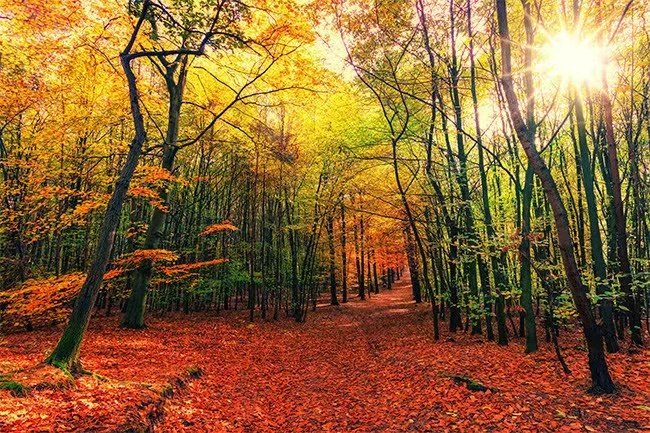
\includegraphics[height=1.5 in]{../pic/pre-quantization.jpg}}
	\hspace{0 pt}
	\subfigure[M = 2]{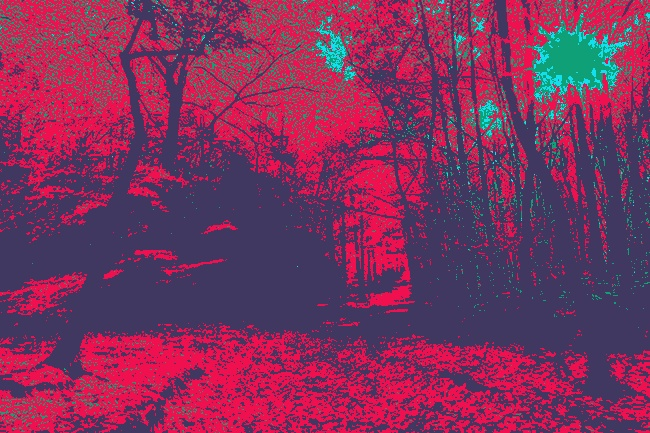
\includegraphics[height=1.5 in]{../pic/new2.jpg}}
	\hspace{0 pt}
	\subfigure[M = 3]{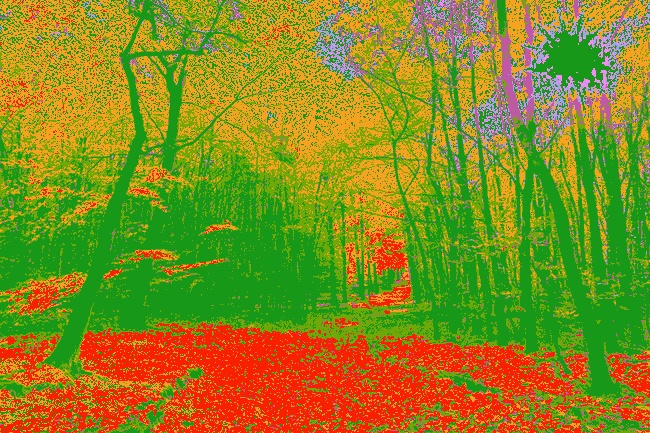
\includegraphics[height=1.5 in]{../pic/new3.jpg}}
	\hspace{0 pt}
	\subfigure[M = 4]{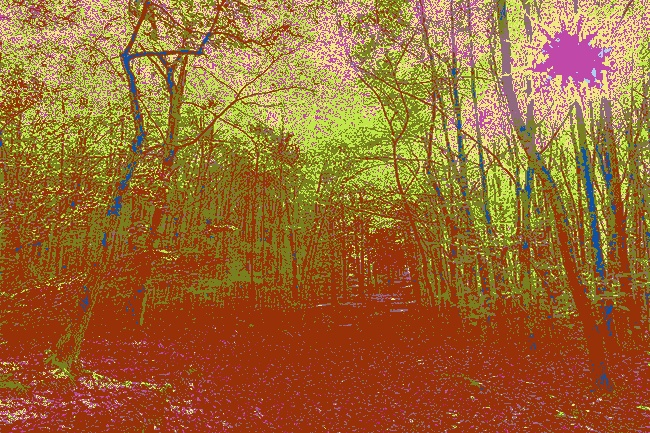
\includegraphics[height=1.5 in]{../pic/new4.jpg}}
	\hspace{0 pt}
	\subfigure[M = 5]{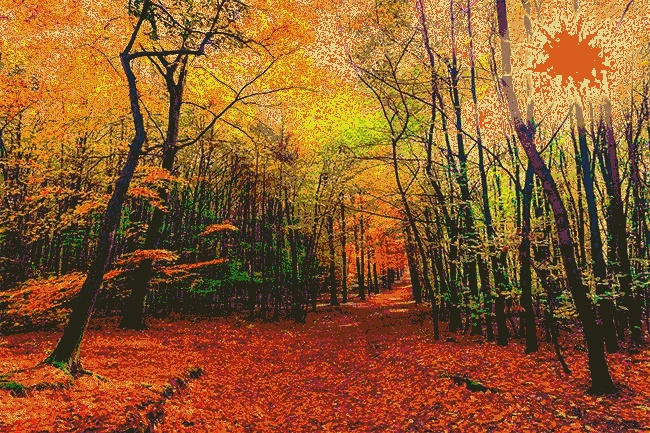
\includegraphics[height=1.5 in]{../pic/new5.jpg}}
	\hspace{0 pt}
	\subfigure[M = 6]{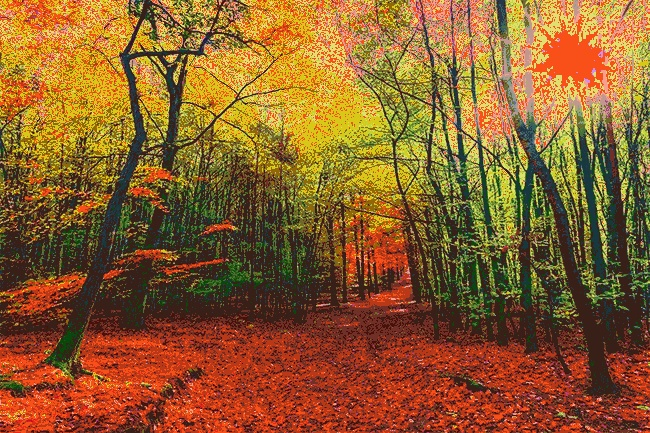
\includegraphics[height=1.5 in]{../pic/new6.jpg}}
	\hspace{0 pt}
	\subfigure[M = 7]{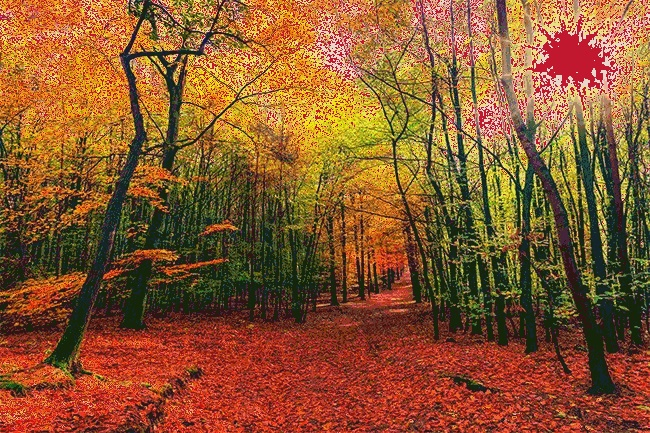
\includegraphics[height=1.5 in]{../pic/new7.jpg}}
	\hspace{0 pt}
	\subfigure[M = 8]{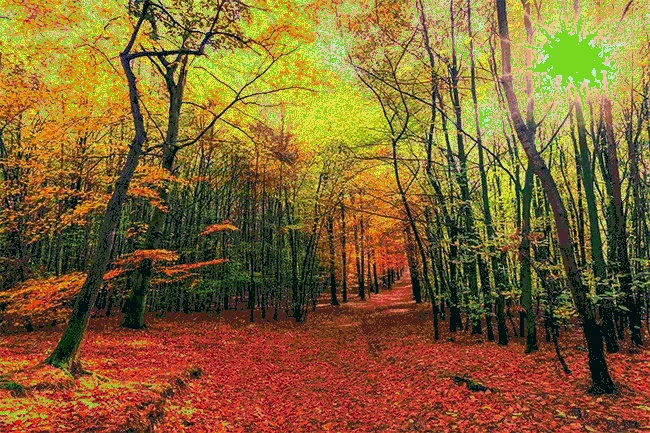
\includegraphics[height=1.5 in]{../pic/old8.jpg}}
	\hspace{0 pt}
	\subfigure[M = 9]{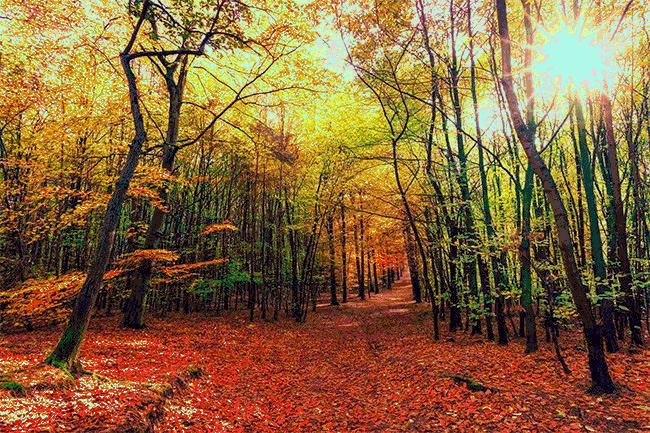
\includegraphics[height=1.5 in]{../pic/old9.jpg}}
	% \hspace{0 pt}
	% \subfigure[M = 10]{\includegraphics[height=1.5 in]{code/new10.jpg}}
	\caption{Pictures after Quantization}
	\label{fig:PicQuant}
\end{figure}

Because when $M > 8$, the code running time is even longer, I am sorry about I cannot give you the left picture in my report.

Through calculation the mean squared error is decreasing when the $M$ is decreasing. The colors in pictures are becoming more and more.

\section{Optimal Quantization Strategy When PDF Has Uniform Distribution}
We have the quantization error of J which can be described as below:
\begin{equation}
J = \sum_{i = 1}^{M}  \int_{b_{i - 1}}^{b_i} [Q_i(x) - x]^2 \, p(x) \; \mathrm{d}x
\end{equation}

In the special case of uniform distribution, we Have
\begin{equation}
J = \sum_{i = 1}^{M}  \int_{b_{i - 1}}^{b_i} [q_i - x]^2 \; \mathrm{d}x
\label{eq:label}
\end{equation}

\subsection{Find the Optimal Quantization Level}

To find the best $q_i$, take the partial derivative of $q_i$
\begin{equation*}
	\begin{aligned}
		\frac{\partial J}{\partial q_i} &= \sum_{i = 1}^{M} \int_{b_{i - 1}}^{b_i} \frac{\partial}{\partial q_i} (q_i^2 - 2q_ix + x^2) \; \mathrm{d}x \\
		&= \sum_{i = 1}^{M} \int_{b_{i - 1}}^{b_i} (2 q_i - 2x) \; \mathrm{d}x \\ 
	\end{aligned}
\end{equation*}

We want $\frac{\partial J}{\partial q_i} = 0$. Therefore \\ 
\begin{equation*}
	\begin{aligned}
		 q_i \int_{b_{i - 1}}^{b_i} \; \mathrm{d}x &=  \int_{b_{i - 1}}^{b_i} x \; \mathrm{d}x \\ 
		 q_i (b_i - b_{i - 1}) &= \frac12 \;  (b_i^2 - b_{i - 1}^2) 	 
	\end{aligned}
\end{equation*}

Therefore
\begin{equation}
	q_i = \frac{b_i + b_{i - 1}}{2} 
	\label{eq:qiResult}
\end{equation}

\subsection{Find the Optimal Quantization Interval}

And, the same as the $q_i$, take the partial of $b_i$, and make $\frac{\partial J}{\partial b_i} = 0$
\begin{equation*}
	\begin{aligned}
		\frac{\partial J}{\partial b_i} &= \frac{\partial}{\partial b_i} \sum_{i = 1}^{M} \int_{b_{i - 1}}^{b_i} (q_i - x)^2 \; \mathrm{d}x \\ 
		&= \frac{\partial}{\partial b_i} [\int_{b_{i - 1}}^{b_i} (q_i - x)^2 \; \mathrm{d}x + \int_{b_{i}}^{b_{i + 1}} (q_{i + 1} - x)^2 \; \mathrm{d}x] \\ 
		&= 0
	\end{aligned}
	\label{eq:biCondi}
\end{equation*}

We learned (\ref{eq:derivation}) in out freshman year that
\begin{equation}
\begin{aligned}
	\frac{d}{dx} \int_{a}^{x} \, f(t) \; \mathrm{d}t &= f(x) \\ 
	\frac{d}{dx} \int_{x}^{a} \, f(t) \; \mathrm{d}t &= - f(x)
\end{aligned}
\label{eq:derivation}
\end{equation}

Rewrite the (\ref{eq:biCondi})
\begin{equation*}
	\begin{aligned}
		(q_i - b_i)^2 &= (q_{i + 1} - b_i)^2 \\ 
		b_i - q_i &= q_{i + 1} - b_i
	\end{aligned}
\end{equation*}

We can have the other result
\begin{equation}
	b_i = \frac{q_{i + 1} + q_i}{2}
	\label{eq:biResult}
\end{equation}

\subsection{Conclude the Optimal Quantization Strategy}

If we combine (\ref{eq:qiResult}) with (\ref{eq:biResult}). First, we can know that 
\begin{gather}
	q_i = \frac{b_i + b_{i - 1}}{2} \notag \\ 
	q_{i + 1} = \frac{b_{i + 1} + b_i}{2} \notag
\end{gather}

Put them in (\ref{eq:biResult})
\begin{equation*}
	\begin{aligned}
		b_i &= \frac{q_i + q_{i + 1}}{2} \\ 
		&= \frac{1}{2} \; (b_i + \frac{b_{i - 1} + b_{i + 1}}{2}) \\ 
	\end{aligned}
\end{equation*}

Therefore
$$
	b_i = \frac{b_{i - 1} + b_{i + 1}}{2}
$$

We can easily know that $b_i$ is an arithmetic sequence, and because (\ref{eq:qiResult}), $q_i$ is an arithmetic sequence too. 

In conclusion, if $p(x)$ is in the special case of uniform distribution, the range of $[0, 1]$ should be equally divided into M parts, and $q_i$ should be the mean of $b_i$ and $b_{i + 1}$.

\bibliographystyle{ieeetr}
\bibliography{../bib/database}

\begin{appendices}
\section{Code Listing}
\begin{python}
from cv2 import imread, imwrite
import numpy as np

img_ = imread("../../pic/picForQuantization.jpg")
X, Y, _ = img_.shape
M = 2 # M in 2 to 10

cx = np.zeros(256)
cy = np.zeros(256)
cz = np.zeros(256)
intv = np.arange(0, 256, 1)

X, Y, _ = img_.shape

img = np.zeros((X, Y, 3))
for x in range(X):
    for y in range(Y):
        for z in range(3):
            img[x, y, z] = int(round(img_[x, y, z]/8))

ppp = np.fromfile("P.bin")
P_  = np.reshape(ppp, (256, 256, 256))
P = np.zeros((33, 33, 33))
for i in range(32):
    for j in range(32):
        for k in range(32):
            P[i, j, k] = np.average(P_[8*i:8*i + 8, 8*j:8*j + 8, 8*k:8*k + 8])

def updateB(Q, B):
    for i in range(32):
        for j in range(32):
            for k in range(32):
                dis = [(i - q[0])**2 + (j - q[1])**2 + (k - q[2])**2 for q in Q]
                B[i, j, k] = np.argmin(dis)

def updateQ(P, B):
    num = np.zeros((2**M, 3))
    den = np.zeros((2**M, 3))
    for i in range(32):
        for j in range(32):
            for k in range(32):
                num[int(B[i][j][k])] += P[i][j][k] * np.array([i, j, k])
                den[int(B[i][j][k])] += P[i][j][k]
    Q = num/den

def quantiz(img, B, Q):
    qimg = np.zeros((X, Y, 3))
    for x in range(X):
        for y in range(Y):
            qimg[x][y] = (Q[int(B[int(img[x][y][0]), int(img[x][y][1]), int(img[x][y][2])])])
    return qimg

def judge(img, qimg):
    err = 0
    for x in range(X):
        for y in range(Y):
            err += (img[x, y, 0] - qimg[x, y, 0])**2 + (img[x, y, 1] - qimg[x, y, 1])**2 + (img[x, y, 2] - qimg[x, y, 2])**2
    return err

Q = np.random.randint(0, 32, size=(2**M, 3))
B = np.zeros((33, 33, 33))

flag = 0
err = 1
for it in range(30):
    print(it)
    updateB(Q, B)
    updateQ(P, B)
qimg = quantiz(img, B, Q)
err = judge(img, qimg)
print(err)

imwrite("new" + str(M) + ".jpg", qimg*8)
imwrite("img.jpg", img)
\end{python}
\end{appendices}

\end{document}